	\begin{mydef}
		
		\iftoggle{eleve}{%
			Si une figure et \hrulefill
			
			\vspace*{0.2cm}
			\hrulefill
			
			\vspace*{0.2cm}
			\hrulefill
		}{%
			Si une figure et son symétrique par rapport à une droite $(d)$ sont confondus, alors $(d)$ est un \kw{axe de symétrie} de la figure.
		}
		
	\end{mydef}

	\begin{myexs}
		\begin{center}
			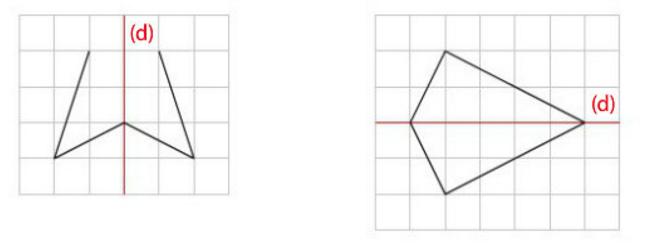
\includegraphics[scale=0.75]{axes}
		\end{center}
	\end{myexs}

	\begin{mydef}
		\iftoggle{eleve}{%
			Si une figure et \hrulefill
			
			\vspace*{0.2cm}
			\hrulefill
			
			\vspace*{0.2cm}
			\hrulefill
		}{%
			Si une figure et son symétrique par rapport à un point $O$ sont confondus, alors $O$ est un \kw{centre de symétrie} de la figure.
		}
	\end{mydef}

	\begin{myexs}
		\begin{center}
			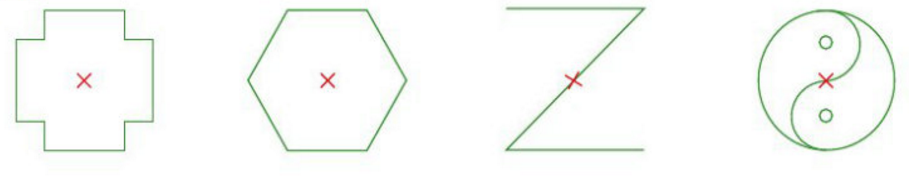
\includegraphics[scale=0.6]{centres}
		\end{center}
	\end{myexs}


%	\begin{myapp}
%		Dire si les panneaux suivants ont un axe et / ou un centre de symétrie.
%		
%		\begin{center}
%			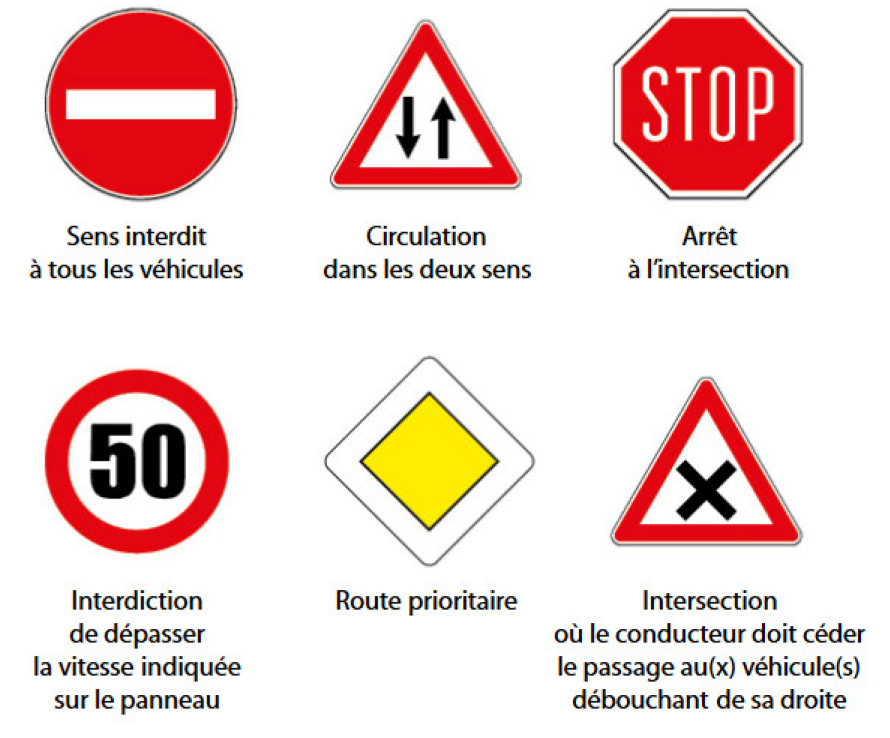
\includegraphics[scale=0.43]{app}
%		\end{center}
%	\end{myapp}